\documentclass[12pt]{article}

\usepackage{scicite,times,graphicx,float,hyperref}
\usepackage[skip=0pt]{caption}
\usepackage[utf8]{inputenc}
\usepackage{enumitem}
\usepackage{booktabs}

\topmargin -1.0cm
\oddsidemargin 0.0cm
\textwidth 16cm 
\textheight 23cm
\footskip 1.0cm

\newenvironment{sciabstract}{%
\begin{quote} \bf}
{\end{quote}}

\newcounter{lastnote}
\newenvironment{scilastnote}{%
  \setcounter{lastnote}{\value{enumiv}}%
  \addtocounter{lastnote}{+1}%
  \begin{list}%
  {\arabic{lastnote}.}
  {\setlength{\leftmargin}{.22in}}
  {\setlength{\labelsep}{.5em}}
}
{\end{list}}

\title{A Kafka-Based Centralized Platform\\for Smart Vehicle Supervising} 

\author
{Filipe Pires [85122], João Alegria [85048]\\
\\
Software Architecture\\
\normalsize{Department of Electronics, Telecommunications and Informatics}\\
\normalsize{University of Aveiro}\\
} 

\date{\today{}}

%%%%%%%%%%%%%%%%% END OF PREAMBLE %%%%%%%%%%%%%%%%

\begin{document} 

\baselineskip18pt

\maketitle 

\section*{Introduction} %%%%%%%%%%%%%%%%%%%%%%%%%%%%%%%%%%%%%%%%%%%%%%%%%%%%%%%%%%%%%%%%%%%%%%%%%%%%%%%%%%%%%%%%%%%%%%%%%%%%%%%%%%%%%%%%%%%%%%%%%%%%%%%%%%%%%%%%

This report aims to describe the work developed for the second assignment of the course of 'Software Architecture', focused on a platform that collects and 
processes information from simulated vehicles.

....................

We also mention how the work was distributed amongst the authors.
All code developed is publicly accessible in our GitHub repository:
\url{https://github.com/FilipePires98/AS/}.
\newpage

% \vspace{-10pt}
% \begin{itemize}[noitemsep]
%   \item Prepare - the selected farmers move to a Standing Area, ready for orders.
%   \item Start - the actual simulation begins and farmers start moving.
%   \item Collect - farmers collect corn cobs from the Granary (where the cobs initially are).
%   \item Return - farmers return to the Storehouse with the collected corn cobs.
%   \item Stop - farmers stop whatever they are doing and return to the Storehouse.
%   \item Exit - simulation ends and the program closes.
% \end{itemize}
% \vspace{-10pt}

% \begin{figure}[H]
%   \centering
%   \begin{minipage}{\textwidth}
%     \centering
%     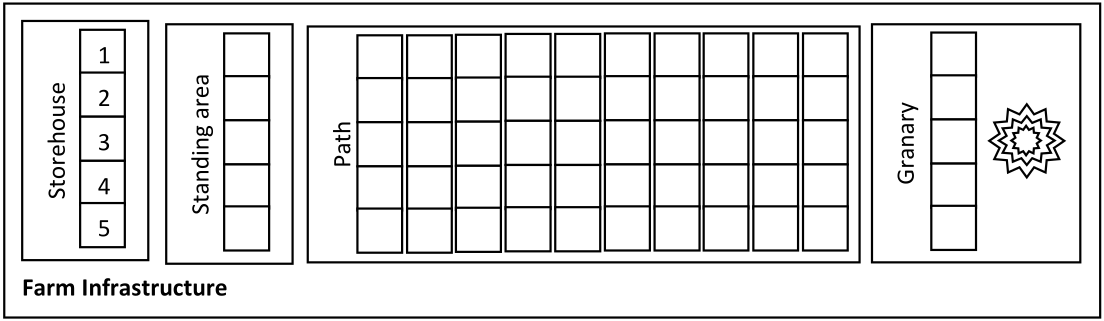
\includegraphics[width=\linewidth]{img/Design_FI.png}
%   \end{minipage}%
%   \caption{Visual representation of the farm, taken from \cite{assign}.}
%   \label{Design_FI}
% \end{figure} 

%\texttt{java -cp <userdir>/build/classes fi.FarmInfrastructure}

\section{IoT, Kafka and Connected Devices} %%%%%%%%%%%%%%%%%%%%%%%%%%%%%%%%%%%%%%%%%%%%%%%%%%%%%%%%%%%%%%%%%%%%%%%%%%%%%%%%%%%%%%%%%%%%%%%%%%%%%%%%%%%%%%%%%%%%%

Internet of Things (IoT) is becoming an increasing topic of interest among technology giants and business communities.
IoT Components are interconnected devices over a network, which are embedded with sensors, software and smart applications so they can collect and exchange data 
with each other or with cloud / data centers.

One of the areas in which IoT is paving its way is the connected vehicles. 
According to Gartner predictions \cite{gartner}, by this year there should be about a quarter-billion connected vehicles on the road, which are more automated, 
providing new in-vehicle services such as enhanced navigation system, real-time traffic updates, weather alerts and integration with monitoring dashboards. 
In order to process the data generated by IoT connected vehicles, data is streamed to central processors usually located in the cloud. 
The collected information can be analysed and data can be extracted and transformed to the final result, which can be sent back to the vehicle or to a monitoring dashboard. 

In this project we explore a hypothetical use case where communication between devices (or entities) is done through Kafka.
Apache Kafka \cite{kafka} is high-throughput distributed messaging system in which multiple producers send data to Kafka cluster and which in turn serves them to consumers. 
It is a distributed, partitioned, replicated commit log service.
The Java application we developed and that is described in this report is a simplified version of an IoT data processing and monitoring application for connected
vehicles, aimed to to explore Kafka capabilities for messaging between entities.

\subsection{The Data} %%%%%%%%%%%%%%%%%%%%%%%%%%%%%%%%%%%%%%

As having actual connected vehicles with processing units capable of collecting car data and transmitting it to other entities was out of the scope of the project, 
this is simulated through a simple text file containing one transmission (or message) per line.
This data file with the name of \texttt{CAR.txt} is placed under a specific directory and is read by our system for processing.

In order to dynamically generate such source data, we developed a small script in Python that receives as parameters the number of cars to be simulated and the 
total number of messages to be generated from those cars and stored in the text file.
The script is called \texttt{generateCAR.py} and is placed in the scripts package inside our project.
By default, it creates 10 different cars and writes 100 messages, but these numbers can be easily modified inside the script. 

We used a random-based approach to generate each aspect of a message.
Unique register codes are created to represent vehicles, as well as their status and speeds.
Message types are not generated with a specific pattern, but we made it far more likely to generate a message of type HEARTBEAT (see section \ref{messages}) 
than of any other type.

%A car is characterized by a register code NN-XX-NN, where N is a number between 0 and 9 and X is a letter from the alphabet in uppercase, so we merely compute 
%random numbers within that range and random indexes from 0 to the size of the used alphabet and build register codes. 
%These codes are validated (ensured to be unique) before adding them to an array of car codes.
%Message types are also determined randomly, although some types are made more likely than others, as well as message timestamps, car speeds and car status values.
%The maximum period between messages is of 5 seconds, although this number is also easily configurable inside the script.
%The maximum car speed is of 150 Km per hour and it is assumed that they are only allowed to drive at up to 120 Km per hour.

\subsection{The Messages} \label{messages} %%%%%%%%%%%%%%%%%

Messages can be of 1 of 3 types, each with a specific purpose and format:

\vspace{-10pt}
\begin{itemize}[noitemsep]
  \item HEARTBEAT - the simplest type of message meant to notify the system that the car is still connected. \\ Format: $|$ car\_reg $|$ timestamp $|$ 00 $|$
  \item SPEED - message meant to inform the system about the current speed of the car. This allows the system to determine whether the car is going under the speed limit or not and trigger an alarm if necessary. \\ Format: $|$ car\_reg $|$ timestamp $|$ 01 $|$ speed $|$
  \item STATUS - messages meant to detect whether the smart sensor detects any malfunction. This in theory could help the system provide or suggest a solution for the malfunction to the car driver considering the entire network of connected vehicles. \\ Format: $|$ car\_reg $|$ timestamp $|$ 02 $|$ status $|$
\end{itemize}
\vspace{-10pt}
The car\_reg corresponds to the register code of each vehicle and the timestamp corresponds to the time instance when the message was created, the remaining 
elements are self explanatory.
As we will see, each message type is treated differently both in their purpose and in the care with which their transmission is done. \\
  
$|$ 45-SH-72 $|$ 1586183268975 $|$ 02 $|$ OK $|$

$|$ 28-MC-82 $|$ 1586183269976 $|$ 02 $|$ OK $|$

$|$ 42-UW-71 $|$ 1586183272978 $|$ 00 $|$

$|$ 73-FD-20 $|$ 1586183273979 $|$ 00 $|$

$|$ 28-MC-82 $|$ 1586183274980 $|$ 01 $|$ 20 $|$

$|$ 55-LZ-42 $|$ 1586183276981 $|$ 00 $|$

$|$ 64-IY-98 $|$ 1586183281986 $|$ 00 $|$

$|$ 45-SH-72 $|$ 1586183286989 $|$ 00 $|$

$|$ 42-UW-71 $|$ 1586183311005 $|$ 00 $|$

$|$ 80-DE-01 $|$ 1586183315006 $|$ 00 $|$

$|$ 30-UU-59 $|$ 1586183319009 $|$ 00 $|$

$|$ 78-ST-77 $|$ 1586183324009 $|$ 00 $|$

$|$ 28-MC-82 $|$ 1586183325011 $|$ 02 $|$ KO $|$

$|$ 30-UU-59 $|$ 1586183327012 $|$ 01 $|$ 0 $|$

$|$ 73-FD-20 $|$ 1586183328012 $|$ 01 $|$ 130 $|$

Example of a portion of the \texttt{CAR.txt} file.

\newpage 
\section{System Architecture} %%%%%%%%%%%%%%%%%%%%%%%%%%%%%%%%%%%%%%%%%%%%%%%%%%%%%%%%%%%%%%%%%%%%%%%%%%%%%%%%%%%%%%%%%%%%%%%%%%%%%%%%%%%%%%%%%%%%%%%%%%%%%%%%%%

.........................

\subsection{Entities} %%%%%%%%%%%%%%%%%%%%%%%%%%%%%%%%%%%%%%

% description of each
% block diagram
...

\subsection{Components} %%%%%%%%%%%%%%%%%%%%%%%%%%%%%%%%%%%%

% responsibilities of each
% other diagrams
...

\subsection{User Interface} %%%%%%%%%%%%%%%%%%%%%%%%%%%%%%%%

...

\newpage
\section{Kafka Infrastructure} %%%%%%%%%%%%%%%%%%%%%%%%%%%%%%%%%%%%%%%%%%%%%%%%%%%%%%%%%%%%%%%%%%%%%%%%%%%%%%%%%%%%%%%%%%%%%%%%%%%%%%%%%%%%%%%%%%%%%%%%%%%%%%%%%

.........................

\subsection{Initialization and Destruction Scripts} %%%%%%%%

...

\subsection{Topics and Constraints} %%%%%%%%%%%%%%%%%%%%%%%%

...

\newpage
\section{Additional Remarks} %%%%%%%%%%%%%%%%%%%%%%%%%%%%%%%%%%%%%%%%%%%%%%%%%%%%%%%%%%%%%%%%%%%%%%%%%%%%%%%%%%%%%%%%%%%%%%%%%%%%%%%%%%%%%%%%%%%%%%%%%%%%%%%%%%%

\subsection{Documentation} %%%%%%%%%%%%%%%%%%%%%%%%%%%%%%%%%

...................

\subsection{Assignment Contributions} %%%%%%%%%%%%%%%%%%%%%%

...................

\section*{Conclusions} %%%%%%%%%%%%%%%%%%%%%%%%%%%%%%%%%%%%%%%%%%%%%%%%%%%%%%%%%%%%%%%%%%%%%%%%%%%%%%%%%%%%%%%%%%%%%%%%%%%%%%%%%%%%%%%%%%%%%%%%%%%%%%%%%%%%%%%%%

........................

\begin{thebibliography}{9} %%%%%%%%%%%%%%%%%%%%%%%%%%%%%%%%%%%%%%%%%%%%%%%%%%%%%%%%%%%%%%%%%%%%%%%%%%%%%%%%%%%%%%%%%%%%%%%%%%%%%%%%%%%%%%%%%%%%%%%%%%%%%%%%%%%%%
  \bibliographystyle{Science}

  \bibitem{assign}
    Óscar Pereira,
    \textit{SA: Practical Assignment no.2},
    University of Aveiro,
    2019/20.
  
  \bibitem{gartner}
    Smarter With Gartner,
    \textit{Staying on Track with Connected Car Security},
    \url{https://www.gartner.com/smarterwithgartner/staying-on-track-with-connected-car-security/},
    accessed in April 2020.

  \bibitem{kafka}
    Apache Kafka,
    \textit{Apache Kafka: A Distributed Streaming Platform},
    \url{https://kafka.apache.org/},
    acessed in April 2020.

  % \bibitem{uml}
  %   Object Management Group,
  %   \textit{What is UML},
  %   \url{https://www.uml.org/what-is-uml.htm},
  %   accessed in March 2020.
    
  % \bibitem{javadoc}
  %   Oracle,
  %   \textit{Javadoc Technology},
  %   \url{https://docs.oracle.com/javase/8/docs/technotes/guides/javadoc/index.html},
  %   accessed in February 2020.

\end{thebibliography}

\clearpage

\end{document}




















